\documentclass[conference]{IEEEtran}
\IEEEoverridecommandlockouts
% The preceding line is only needed to identify funding in the first footnote. If that is unneeded, please comment it out.
\usepackage{cite}
\usepackage{amsmath,amssymb,amsfonts}
\usepackage{algorithmic}
\usepackage{graphicx}
\usepackage{textcomp}
\usepackage{xcolor}
\usepackage{url}
\newcommand\BibTeX{B{\sc ib}\TeX}

\begin{document}

\title{Survey on Training Large Language Models using Parallel Processing\\
	\author{\IEEEauthorblockN{Haoran Wang}
		\IEEEauthorblockA{University of Oregon}
		\IEEEauthorblockA{CIS 631 (Parallel Processing), Fall 2020}
	}
}

\maketitle

\begin{abstract}
Language models, especially neural language models are very important to Natural Language Processing. These powerful neural language models, such as BERT have started a revolution in NLP research. Researchers can fine-tune the pre-trained BERT models and achieve state-of-the-art result in many NLP tasks. However, these powerful models also come with a steep price to pay in terms of the computational cost during training. BERT has 330 million parameters and it takes months to train the BERT-large model with a single GPU and days on a cluster of GPUs. In fact, when Google published BERT, it took them 4 days to train on 16 Cloud TPUs. Therefore, parallel processing is crucial to speedup the training process of these large language models. This survey summarizes how parallelism is applied when training a large language model such as BERT. This survey examines this topic from three perspectives, parallel architecture, data parallelism, as well as hardware specialization.
\end{abstract}

\section{Introduction}
Natural Language Processing (NLP) is the study of how to make computers understand human languages. The core component of modern NLP are language models, they power the popular NLP application such as Amazon Alexa and Google Assistant. Language models determine the probability of the next word by analyzing the text in data. Take speech recognition task for example, when analyzing homophone phrases such as "but her" and "butter", a language model will take the context of the sentence and tell Alexa which one sounds more natural and makes more sense.\\

There are two kinds of language models, statistical and neural. They corresponds to statistical based machine learning and deep learning. Statistical language models, such as N-grams \cite{ngram} predicts the last word in a sequence based on the context of N-1 words. Those statistical language models require a lot of feature engineering and are considered too simple compared to neural language models by today's standard. On the other hand, neural language models are based on neural networks that can capture more context and dependencies from the language. Since language is significantly complex and keeps evolving, the more complex the language models are, the better they would be at performing NLP tasks.\\

One particular language model, BERT (Bidirectional Encoder Representation from Transformers) \cite{BERT} has taken the NLP landscape by storm. BERT was created by Google AI Language lab in 2018. Since then, BERT has been able to achieve state-of-the-art results in a wider variety of NLP benchmark datasets, such as GLUE\cite{glue}. BERT is a very large language model. It was trained on 3.3 billion words from Wikipedia using 16 Google's Cloud TPUs. This would simply not happen without the help of parallel processing.\\

However, parallel processing does not come naturally to NLP because of its sequential nature. This survey introduces the challenges and solution to train large language models in parallel.\\

\begin{itemize}
	\item Parallel Architecture - Since each word in the sequence depends heavily on its context (other words in the sequence), they cannot be trained in parallel without changing the model's architecture to make them independent of each other.
	\item Data Parallelism - Since an enormous amount of data is needed to train the model, they could become performance bottleneck. Therefore,  batch size needs to be optimized to fully utilize the memory bandwidth while maintaining accuracy.
	\item Hardware Specialization - Application Specific Integrated Circuit (ASIC) such as TPUs are designed specifically for training deep learning models. They are more efficient and cost less than GPUs.
\end{itemize}

\section{Background} 
	\subsection{BERT}
	BERT, short for Bidirectional Encoder Representation from Transformers has two pre-trained models: BERT base and BERT large. BERT base has 12 layers, and around 110 million parameters. BERT large has 24 layers, and around 340 million parameters \cite{BERT}.\\
	
	\subsection{Transformer}
	To understand BERT, we need to first understand how Transformers work. BERT is basically layers of bidirectional Transformers. Each transformer consist of a number of encoders and decoders. Each encoder and decoder has two layers: a multi-headed attention layer and a fully connected feed-forward neural network.\\
	
	\begin{figure}[!htbp]
		\centering
		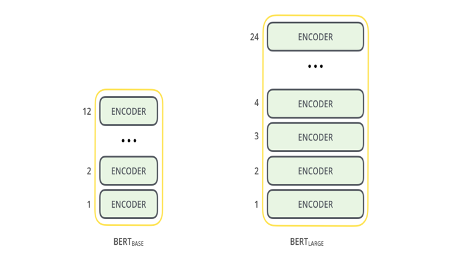
\includegraphics{figures/figure1.png}
		\caption{\label{fig:my-label} BERT base and BERT large \cite{BERT}}
	\end{figure}

	\begin{figure}[!htbp]
		\centering
		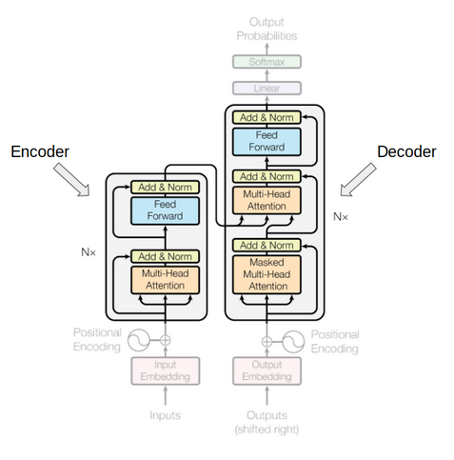
\includegraphics{figures/figure2.png}
		\caption{\label{fig:my-label} Transformer Architecture \cite{BERT}}
	\end{figure}
	
	Multi-headed attention layer computes self-attention multiple times in parallel and independently. The outputs are then concatenated and linearly transformed.\\
	
	\subsection{Self-attention}
	“Self-attention, sometimes called intra-attention, is an attention mechanism relating different positions of a single sequence in order to compute a representation of the sequence. \cite{attention}” Therefore, it helps the encoder to look at other words in the input sentence when encoding each word. Thus, it makes the encoder take the contexts of the sentence into consideration.\\
	
	\begin{figure}[!htbp]
		\centering
		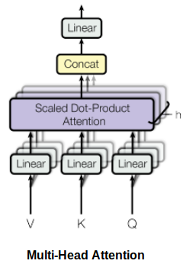
\includegraphics{figures/figure3.png}
		\caption{\label{fig:my-label} Multi-Head Attention \cite{attention}}
	\end{figure}
	
	To calculate self-attention, the encoder creates a query vector, a key vector, and a value vector for the embeddings of different words in the sequence. Next, it calculates the dot product of the query vector with the key vector for each word of the input sequence against the other words in the sequence. Then, it divides the dot product by the square root of the dimension of the key vectors, followed by an application of the softmax function. Finally it multiplies each value vector by the softmax score and sums up the weighted value vectors.\\
	
	\begin{figure}[!htbp]
		\centering
		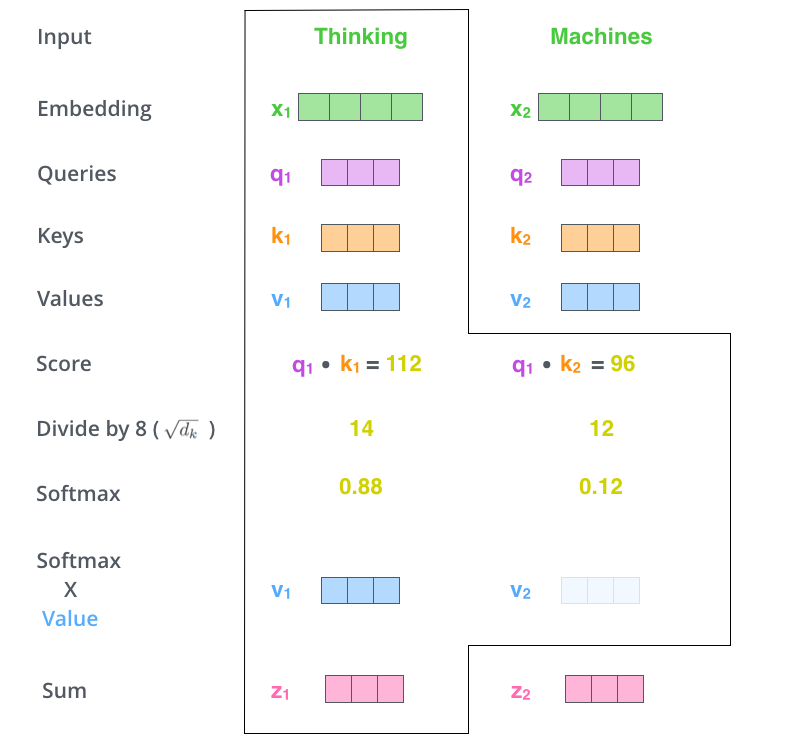
\includegraphics[scale=0.3]{figures/figure4.png}
		\caption{\label{fig:my-label} Calculate Self-Attention \cite{self-attention}}
	\end{figure}
		
	\subsection{Google Cloud TPUs}
	Tensor Processing Units (TPUs) are Google's custom developed ASICs used to accelerate machine learning workloads, especially deep neural network training \cite{TPU-1}. Since they are specifically designed as a matrix processor, they can handle the massive multiplications and additions at blazing fast speed while consuming much less power. Google does not sell TPU devices, and only provides them as a Google Cloud computing service.\\
	
	Each TPU core has a scalar, vector, and matrix units (MXU). The MXU provides the bulk of the computer power in a TPU chip. Each MXU can perform up to 16 thousand multiply-accumulate operations in each cycle. While the MXU inputs and outputs are 32-bit floating point values, the MXU performs multiplications at reduced bflaot16 precision. The reason is that bfloat16 representation provides better training accuracy than the IEEE half-precision representation. \cite{TPU-2}\\
	
	\begin{figure}[!htbp]
		\centering
		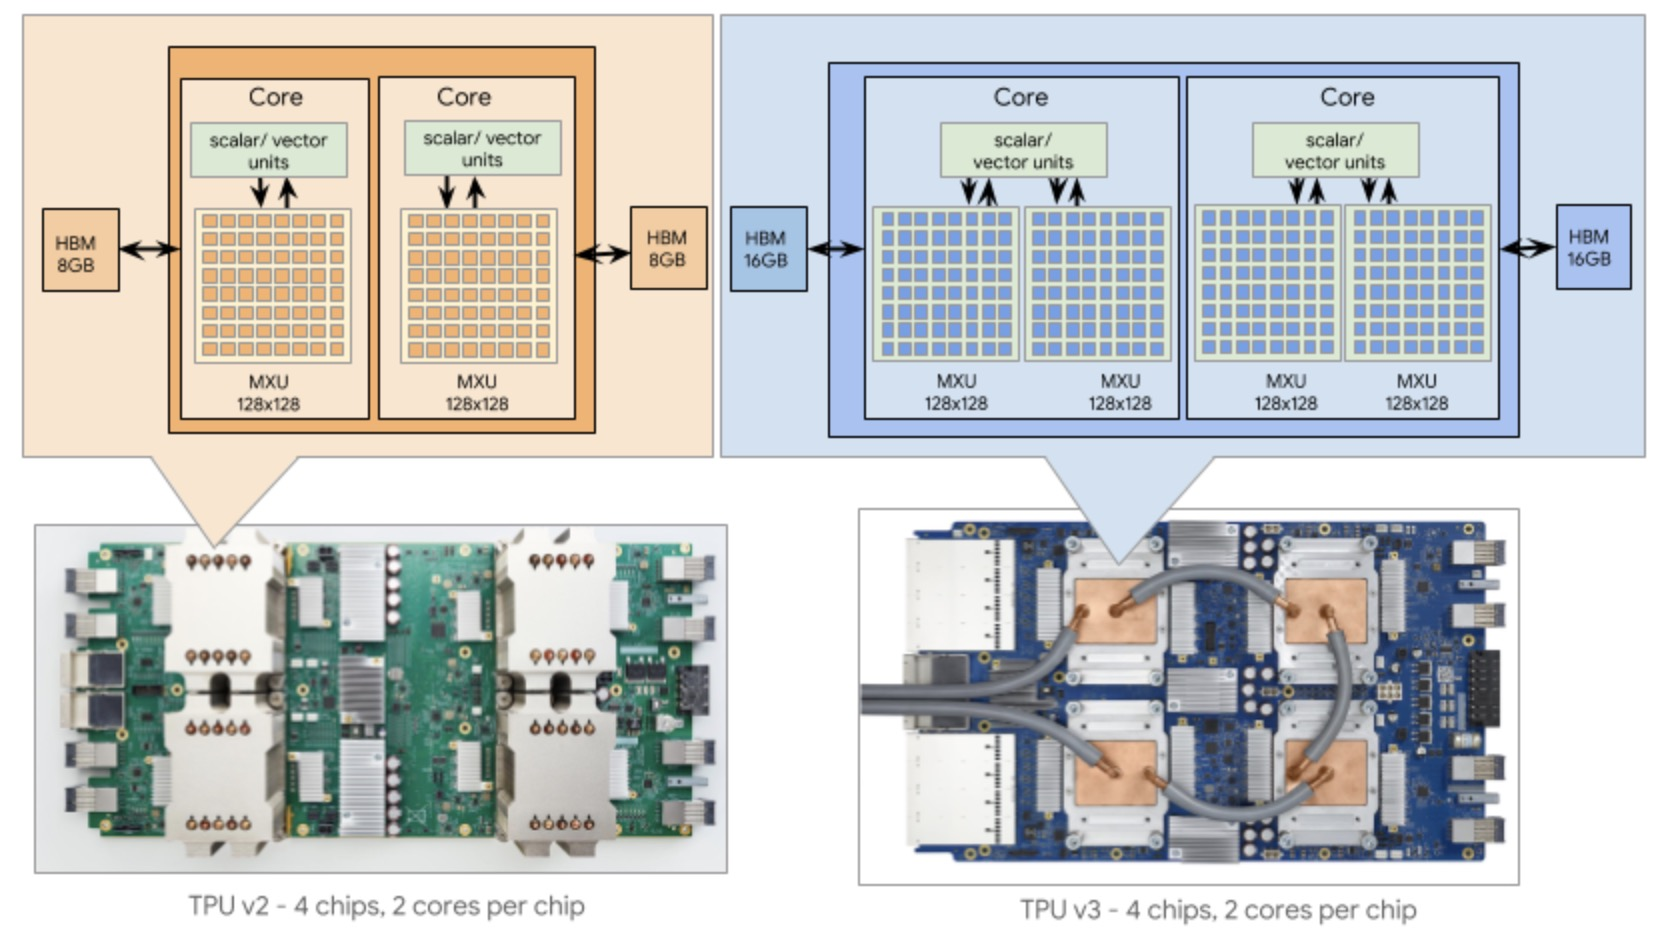
\includegraphics[scale=0.3]{figures/figure5.png}
		\caption{\label{fig:my-label} TPU v2 and TPU v3 \cite{TPU-1}}
	\end{figure}
	
	Google Cloud TPUs are usually configured as TPU pods, which are clusters of TPU devices that are connected through dedicated high-speed networks. The current most powerful TPU is TPU v3, which has 16 GB of high-bandwidth memory (HBM) for each core and one MXU for each core. In a TPU v3 pod configuration, it can have up to 2048 total TPU cores and 32 TB of total HBM.\\
	
\section{Research Review}
	\subsection{Parallel Architecture}
	As introduced in the background section, Transformers are the building blocks of BERT. The Transformer architecture was introduced in the paper "Attention is All You Need" \cite{attention} by Google in 2017. One big motivation for designing this architecture is parallelization when solving sequence to sequence (seq2seq) problems, which is often used for machine translation tasks. However, this task cannot be parallelized easily due to its sequential natural.\\
	
	Seq2seq is one of the common categories of NLP tasks. As the name suggests, both the input and output are sequences. A typical sequence to sequence model has two parts, an encoder and a decoder. Before Transformers, two Recurrent Neural Networks (RNNs) are combined into an Encoder-Decoder model.\cite{RNN}\\
	
	Here is how a typical RNN Encoder-Decoder model works. After each word in the input sequence is converted into a vector by the word embedding. The first vector is fed into the encoder RNN, which results  an output vector. This output vector will then serve as the next input for the encoder RNN. Together with the second vector in the sequence, they are fed into the encoder RNN again to produce another output vector. This process is repeated until all words in the input sequence has been processed. The last output vector, also called context vector is dependent on all of the words in the input sequence, which represents the meaning of the entire input sequence. This context vector will then be the first input to feed into decoder RNN, which will generate the first word of the output sequence. This process of generating and feeding outputs back into the decoder is continued until the end of the sequence has been processed.\\
	
	\begin{figure}[!htbp]
		\centering
		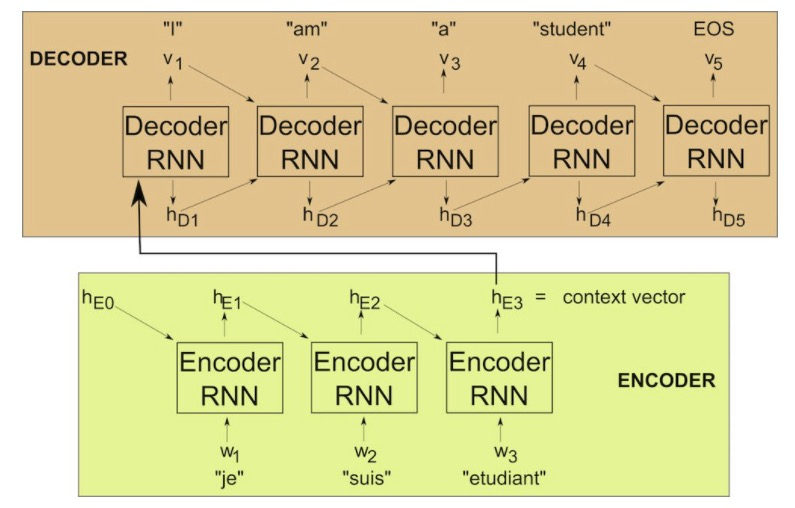
\includegraphics[scale=0.3]{figures/figure6.png}
		\caption{\label{fig:my-label} RNN Encoder-Decoder Architecture \cite{transformer}}
	\end{figure}
	
	This RNN Encoder-Decoder model has been very effective for many NLP tasks. In fact, Google Translate has been using it as a base structure under the hood since the end of 2016\cite{google-translate}. However, RNN Encoder-Decoder has two problems. The first one is that RNN approach does not work well for longer sentences. Since the meaning of the entire input sequence is expected to be captured by a single context vector, it is often considered as nave and thus performs poorly when encoding longer sentences. The second problem is that RNN implementation cannot be parallelized. As the name RNN suggests, it is recurrent, which means it has to wait for the previous step to finish before it can move on to the next one. This lengthens the time to train the model as well as to run inference. Google's Transformer model successfully solved those two problems by adding attention mechanism and dumping the RNN structure. In the next paragraph, I am going to focus on how transformer solves the problem of parallelization.\\
	
	By discarding the sequential nature of RNN, Transformer's encoders can process the words of the input sequence in parallel. For the encoders, the first step is to preprocess the input sequence. There are two parts to be preprocessed. The first part is to use word embeddings to get vector representation of each word, this is common to any modern NLP models. The second part is unique to Transformers, it will encode the position of each word to capture the sequential relationships. Position encoding provides the information on the ordering of the words in the input sequence, this information is then used to calculate self-attention, which captures the relationships between words in the input sequence. By encoding the positions into word vectors, they can capture word relationships while allowing word vectors to be processed by encoder in parallel. This is because the current word vector does not need to wait for the previous word vector to be processed like in RNN. Next, these post processed vectors are fed into two Encoder Self-Attention layers to learn the relationships between different words in the input sequence.\\
	
	For the decoder, the Encoder-Decoder Attention layers and Decoder Self-Attention layers passe the input sequence to generate the output sequence. The hidden states that are the outputs of the encoder are fed into Encoder-Decoder Attention layer, and the previously generated words of the output sequence are fed into Decoder Self-Attention layer. Naturally, the decoder process is sequential, output sequence is generated one word at a time. This is because the Decoder Self-Attention layers rely on previously generated output sequence words. On contrary to RNN Encoder-Decoder, transformer can generate the output sequence in parallel during the training phase by masking. During the training phase, since the output sequences are already available, decoding process can still be parallelized by masking (replacing with zeroes) the appropriate parts of the previously generated output sequences. However, this cannot be done during inference since the output sequence is unknown.\\
	
	\begin{figure}[!htbp]
		\centering
		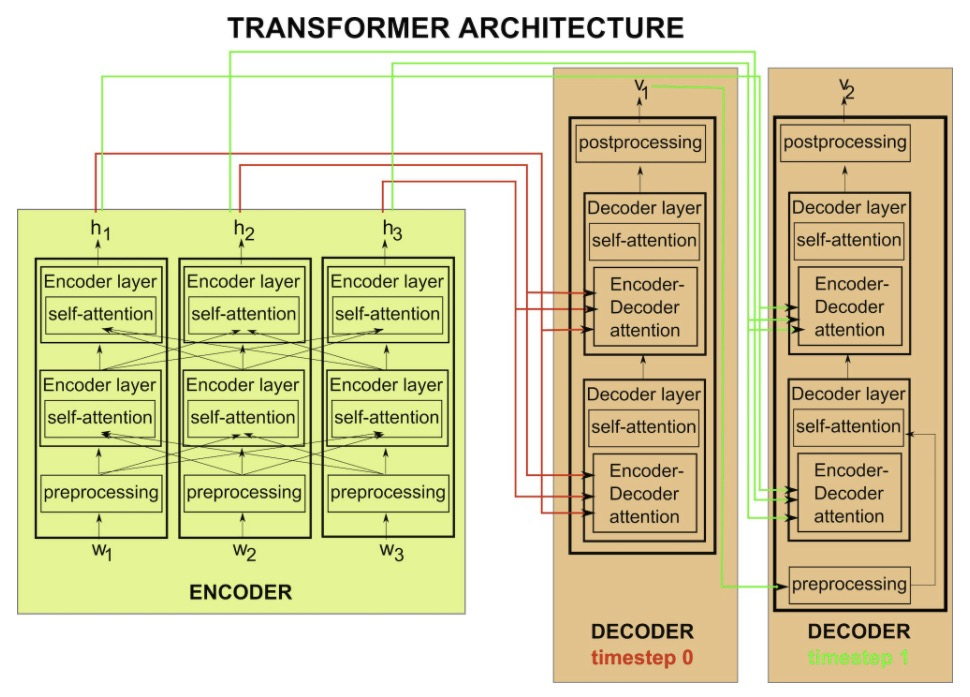
\includegraphics[scale=0.26]{figures/figure7.png}
		\caption{\label{fig:my-label} Transformer Architecture \cite{transformer}}
	\end{figure}
	
	\subsection{Data Parallelism}
	When training neural networks, large batch sizes are usually avoided because they could easily cause models to overfit. In addition, GPU memory runs out quickly when using large batch sizes. However, by increasing batch sizes, one can speedup the training process, since it is the equivalent of taking a few big steps, instead of taking many little steps to minimize loss. The challenge is to increase batch sizes without losing accuracy. This paper \cite{LAMB} managed to scale the batch size of BERT to the memory limit of a TPU v3 pod without losing accuracy, and reduced the BERT training time from 3 days to around 76 minutes using a layer wise adaptive large batch optimization technique called LAMB (Layer-wise Adaptive Moments optimizer for Batch Training).\\
	
	There are have been extensive research done on large batch optimization. Earlier work found that by carefully hand-tuning hyper-parameters, such as learning rate, one can increase batch size to a certain amount for some problems. One study \cite{krizhevsky2014weird} found that simply scaling the learning rate linearly with respect to the batch size can perform well up to a certain batch size. However, empirical study \cite{shallue2019measuring} shows that learning rate scaling heuristics with the batch size do not hold across all problems or across all batch sizes. More recent works have shifted away from hand-tuning hyper-parameters, and focus on adaptive learning rates for large batch training. Several works have successfully scaled the batch size without degrading the accuracy using adaptive learning rate. \\
	
	The general strategy to adapt learning rate to large batch size training is to normalize the gradient update layer-wise, and scale the learning rate by some factor layer-wise. This paper\cite{LARS} proposed an algorithm called LARS (Layer-wise Adaptive Rate Scaling), which is the basis of LAMB batch optimization for BERT. LARS uses momentum optimizer as the base algorithm. They observed that by using momentum, one can reduce the variance in stochastic gradient descent at the cost of little bias. The LAMB algorithm\cite{LAMB} is obtained by using Adam as the base algorithm. Unlike LARS, LAMB adapts learning to both per dimension normalization with respect to the square root of the second momentum in Adams, as well as layer-wise normalization.\\
	
	To demonstrate the robustness of LAMB, they\cite{LAMB} used very minimal hyper-parameter tuning for the LAMB optimizer. They used the same dataset from the original BERT paper \cite{BERT}, and specifically focused on the SQuAD task in the original BERT paper. They used the F1 score on SQuAD-v1 as the accuracy metric. They maintained the same training procedure as the original paper, except for changing the training optimizer to LAMB. They scaled the batch size from 512 to 32K, which is the memory limit of TPU pod. Their result shows that, by using LAMB optimizer, they achieved F1 score of 91.475, higher than the 90.395 achieved in the original BERT paper. More importantly, they reduced BERT training time from 4 days to around 100 minutes. They achieved 49.1x speedup and 76.7\% efficiency by using the synchronous data parallelism.\\
	
	To obtain further improvements, they \cite{LAMB} used the mixed-batch training with LAMB. BERT training involves two stages, the first 9/10 of the total epochs use sequence length of 128, and the last 1/10 use sequence length of 512. Due to memory limits on TPU, the second stage training can only have maximum batch size of 32K. However, a larger batch size can be used for the first stage because of the shorter sequence length. By using batch size of 64K for the first stage, and 32K for the second stage, they finished BERT training in 76 minutes and 100.2\% efficiency.
	
	\begin{figure}[!htbp]
		\centering
		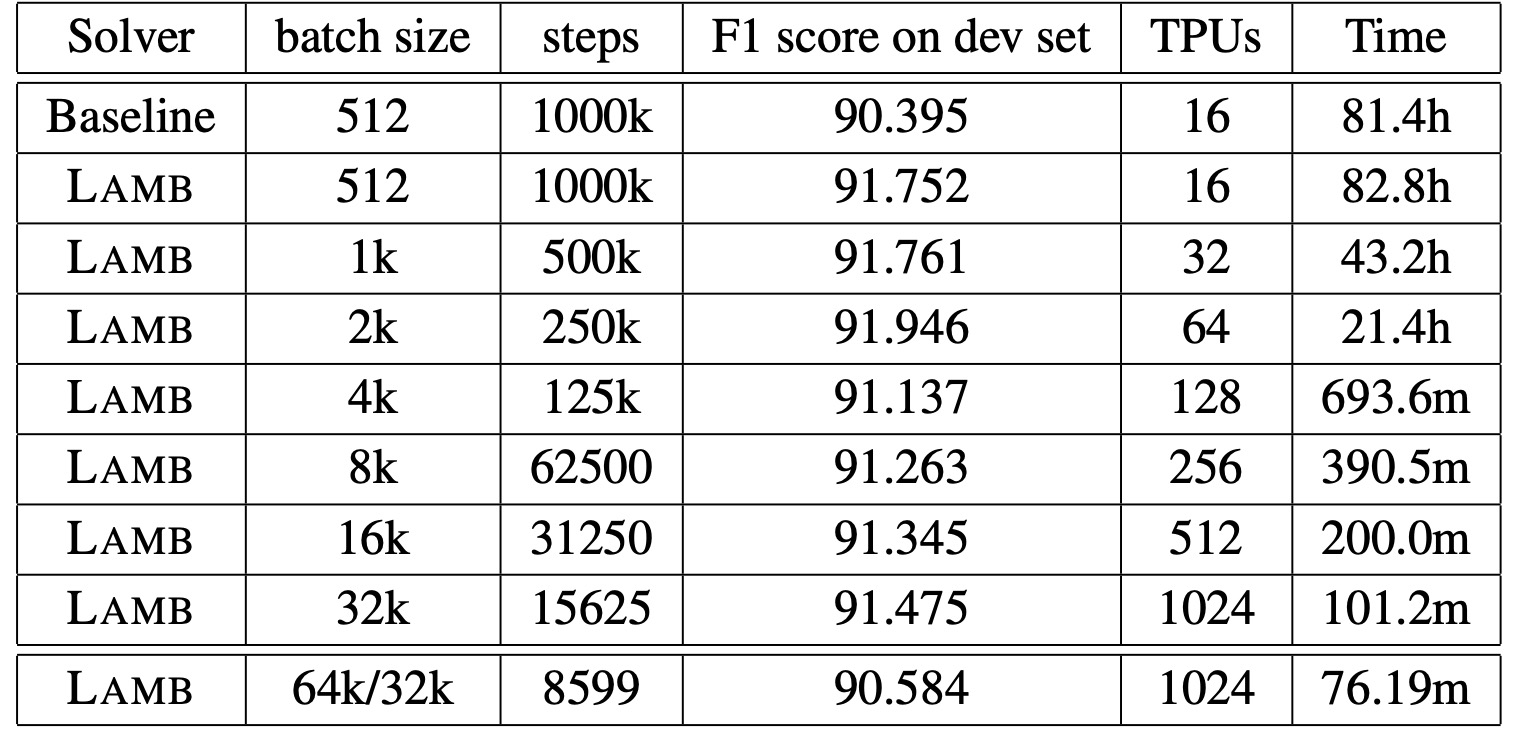
\includegraphics[scale=0.3]{figures/figure8.png}
		\caption{\label{fig:my-label} BERT training with LAMB optimizer \cite{LAMB}}
	\end{figure}
		
	\subsection{Specialization: TPU}
	Hardware specialization is also important in order to achieve good parallel performance. Although GPUs are widely used and achieved good performance in training machine learning models. GPUs are not efficient enough when training a large language model like BERT. In 2016, Google created its own application-specific integrated circuit (ASIC) to support the growing number of speech translations to work with their deep learning framework TensorFlow.\cite{TPUpaper} Experiments have shown that TPUs are about 32\% to 54\% faster for training BERT.\\
	
	The TPU instructions are sent via PCIe Gen3x16 bus into an instruction buffer. Instead of fetching instructions from the CPU, the CPU sends instructions to the buffer.This is intended to keep the matrix unit busy and also reduces the number of pipeline steps required. Once the TPU receives the instructions, it will create a grid of MACs (Multiplier Accumulators) inside the MMU(Matrix Multiply Unit). Each MAC is responsible for multiply, add and accumulate cycle. The MMU performs 8 to 64 bit multiplication and addition on signed and unsigned integers. Then, data is sent via a PCIe Gen3x16 bus to the grid of MACs for execution. The result from the previous layer is passed to the next layer, creating a pipelining. Since get elements from the main memory and load it into the processing unit is the most expensive part in matrix multiplication. By pipelining the output from previous layer as the input into the next layer, it will speedup the matrix multiplication as well as reduce power consumption.\\
	
	\begin{figure}[!htbp]
		\centering
		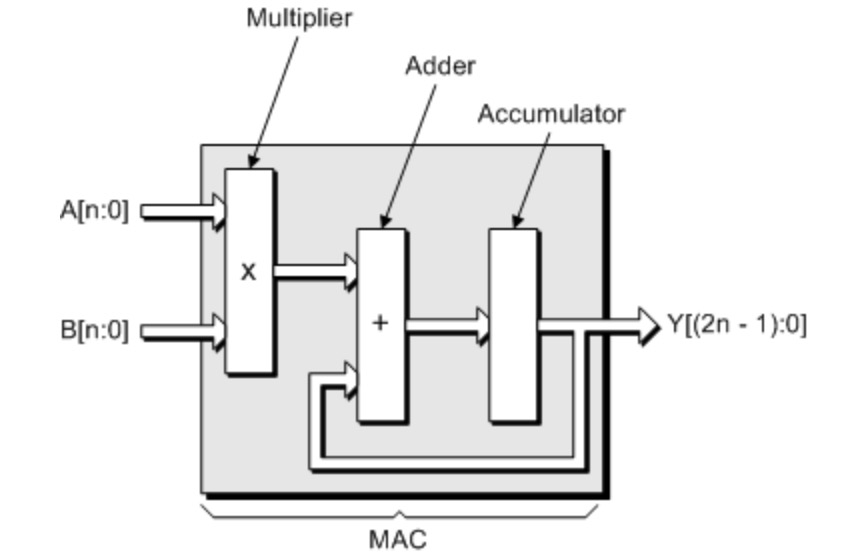
\includegraphics[scale=0.5]{figures/figure9.png}
		\caption{\label{fig:my-label} The core functions forming a MAC \cite{MAC}}
	\end{figure}

	\begin{figure}[!htbp]
		\centering
		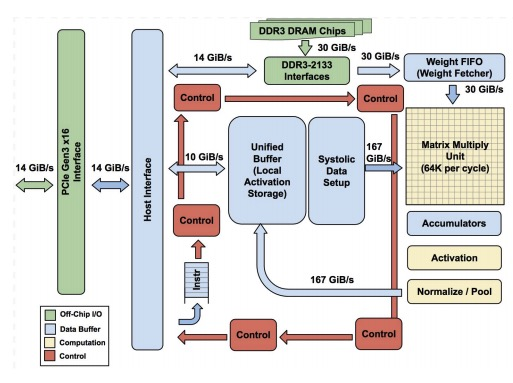
\includegraphics[scale=0.5]{figures/figure10.png}
		\caption{\label{fig:my-label}TPU Block Diagram \cite{TPUpaper}}
	\end{figure}
	
	\begin{figure}[!htbp]
		\centering
		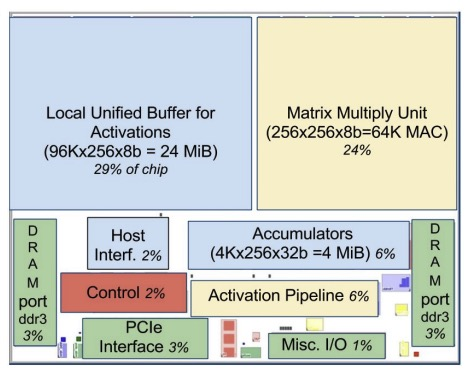
\includegraphics[scale=0.5]{figures/figure11.png}
		\caption{\label{fig:my-label} Floor Plan of TPU die \cite{TPUpaper}}
	\end{figure}
	
	This paper \cite{tpubert} has shown why BERT training on GPUs is slower than TPUs in a theoretical setting. The computational work for BERT training involves 90\% of matrix multiplication. Such as, \(A*B = C\), where A is size of 256x1024 and B is size of 1024x1024. For a TPU, it handles matrix multiplication by splitting the matrix into many smaller matrix tiles of size 128x128 for MACs to execute. This means TPU needs to load 16 matrix tiles from matrix A, and 64 matrix tiles from matrix B for every tile in A, which will result a total of 1024 loads. Assume at 16-bit multiplication, it will be a total of 32MB of data. Assume, the TPU is run at full bandwidth at 600GB/s, this means we need 5.2e-5 seconds to transfer the 32MB of data.\\
	
	For a GPU, it also splits A and B into smaller matrix tiles, but it will use smaller tiles with more processors instead. Take NVIDIA Tesla v100 GPU for example, it will split the matrix into tile size of 96x96 for 16-bit data, and run 160 of those matrix tiles in parallel at full bandwidth with low memory latency. Comparing to TPU's two matrix unites which can hold 128x128 matrices, Tesla v100 has 160 units (80 SMs, 160 thread blocks, each thread block has two 96x96 matrices). To calculate how much time it takes to do the same matrix multiplication above, we can repeat the calculation steps. For matrix A with 256x1024, Tesla will have 33 96x96 tiles; for matrix B, Tesla will have 121 96x96 tiles. In total, 3993 loads of size 96x96 matrix tiles will be needed, for a total of 70MB. Tesla v100 runs at 900GB/s and thus the memory loads will take 7.6e-5 seconds. Therefore, GPU is 32\% slower than TPU in this scenario.\\
	
	This paper \cite{tpubert} also gives insights on how TPU and GPU handle fused operations. TPU can calculate additional element-wise operations such as non-linear activation function or a bias on the fly within a matrix multiplication. This is because TPU does not need to load from global memory as often as GPU, which is expensive. The paper suggests TPU would be 3.2\% faster compared to GPU when doing element-wise operation for a 256x1024 matrix.\\
	
	Finally, this paper \cite{tpubert} examines how 32-bit, 16-bit, and 8-bit multiplication can affect the performance of TPU and GPU. Using the same example above, but the data are now 32-bit values instead of 16-bit. Now, TPU would only needs to load 64x64 matrix tiles. Therefore, it would be 5.3x faster than GPU in theory.\\
	
	\subsection{My Experience}	 
	My recent project involved fine-tuning a XLM-RoBERTa\cite{XLM-ROBERTA} model for multi-lingual toxic comment classification. I trained my model both on GPU and TPU. Since there is no direct support from Google TPU for PyTorch, I used this XLA package \cite{xla} that uses the XLA deep learning compiler to connect PyTorch with Google TPU. My model took around 58 minutes on Tesla V100 and only took around 12 minutes on TPU. This speedup allowed me to further fine-tune my model since I do not need to wait for an hour to see the result.
	
	\begin{table}[!htbp]
		\centering
		\begin{tabular}{|c|c|}
			\hline
			{XLA : 1} & 12m 16s \\ \hline
			{XLA : 2} & 12m 12s \\ \hline
			{XLA : 3} & 12m 15s \\ \hline
			{XLA : 4} & 12m 13s \\ \hline
			{XLA : 5} & 12m 18s \\ \hline
			{XLA : 6} & 12m 17s \\ \hline
			{XLA : 7} & 12m 28s \\ \hline
			{XLA : 8} & 12m 19s \\ \hline
		\end{tabular}
		\caption{\label{table:my-label} Training Time on a TPU using its 8 core}
	\end{table}
	
\section{Conclusion}
	This survey paper discussed how parallel processing is used to help training large language models. Although parallel processing cannot be applied to NLP easily, one can change the model architecture to allow data to be independent from each other. During the training phase, one can use optimizer such as LAMB to achieve data parallelism that can fully utilize available bandwidth. Finally, TPU should be used when training large language models for better speedup and efficiency.

\newpage
\bibliography{survey}\
\bibliographystyle{plain}

\end{document}
